\begin{wrapfigure}[13]{r}{10cm}
  \centering
  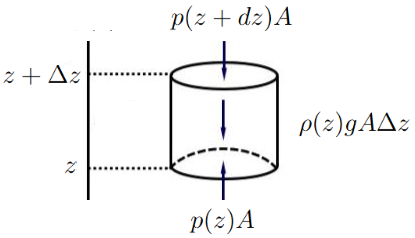
\includegraphics[width=0.5\textwidth]{images/Hinh 7a (S).png}
  \begin{center}
    \figurename{ 7a}
  \end{center}
\end{wrapfigure}

\noindent\textbf{1.} Ở độ cao $z$, áp suất khí quyển là $p(z)$, nhiệt độ là $T(z)$, sử dụng phương trình trạng thái khí lý tưởng, ta tìm được khối lượng riêng của không khí là:
\begin{equation}
  \label{eq:71}
  \rho(z)=\frac{n\mu}{V}=\frac{p{z}\mu}{RT(z)}
\end{equation}
trong đó $n$ là số mol, $V$ là thể tích của khí. Như trong hình 7a, trọng lượng của khí nằm trong một hình trụ bán kính đáy $A$, chiều cao $\Delta z$ ở độ cao $z$ là $\rho(z)gA\Delta z$, mặt trên của hình trụ chịu tác dụng của một lực có độ lớn $p(z+\Delta z)A$ trong khi lực tác dụng lên mặt dưới có độ lớn $p(z)A$. Vì khí bay lên từ từ, các lực tác dụng lên nó phải cân bằng với nhau:
\begin{equation}
  \label{eq:72}
  p(z+\Delta z)A+\rho(z)A\Delta zg=p(z)A
\end{equation}
cho $\Delta z\to 0$, phương trình \eqref{eq:72} có thể được viết dưới dạng:
\begin{equation}
  \label{eq:73}
  \frac{dp}{dz}=-\rho g
\end{equation}
sử dụng phương trình \eqref{eq:71}, ta được:
\begin{equation}
  \label{eq:74}
  \frac{dp}{dz}=-\frac{p\mu g}{RT}
\end{equation}
chia cả hai vế cho $p$, ta có:
\begin{equation}
  \label{eq:75}
  \frac{d\ln p}{dz}=-\frac{\mu g}{RT}
\end{equation}
trong quá trình đoạn nhiệt, $pV^{\gamma}$ là hằng số, theo phương trình trạng thái khí lý tưởng, $p^{1-\gamma}T^{\gamma}$ cũng là hằng số, tức:
\begin{equation}
  \label{eq:76}
  C=-(\gamma -1)\ln{p}+\gamma\ln{T}
\end{equation}
lấy đạo hàm hai vế phương trình \eqref{eq:76} theo $z$ ta có:
\begin{equation}
  \label{eq:77}
  0=-(\gamma - 1)\frac{d\ln p}{dz}+\gamma\frac{d\ln T}{dz}
\end{equation}
sử dụng phương trình \eqref{eq:75}:
\begin{equation}
  \label{eq:78}
  \frac{d\ln T}{dz}=\frac{1}{T}\frac{dT}{dz}=\frac{\gamma-1}{\gamma}\frac{d\ln p}{dz}=-\frac{\gamma -1}{\gamma}\frac{\mu g}{RT}
\end{equation}
vì thế:
\begin{equation}
  \label{eq:79}
  \frac{dT}{dz}=-\frac{(\gamma -1)\mu g}{\gamma R}
\end{equation}
sau khi lấy tích phân, ta nhận được:
\begin{equation}
  \label{eq:710}
  T(z)=T_{0}-\frac{(\gamma-1)\mu g}{\gamma R}z
\end{equation}

\noindent\textbf{2.} Đối với quá trình đoạn nhiệt, $pV^{\gamma}$ là hằng số, do đó ta có thể viết $p=C\rho^{\gamma}$, suy ra:
\begin{equation}
  \label{eq:711}
  v_{s}^{2}=\left(\frac{dp}{d\rho}\right)_{S}=\frac{d(C\rho^{\gamma})}{d\rho}=\gamma C\rho^{\gamma-1}=\gamma\frac{C\rho^{\gamma}}{\rho}=\gamma\frac{p}{\rho}
\end{equation}
thay $\rho=\dfrac{n\mu}{V}$ vào phương trình trạng thái khí lý tưởng $pV=nRT$ để có:

\begin{equation}
  \label{eq:712}
  v_{s}^{2}=\gamma\frac{pV}{n\mu}=\gamma\frac{nRT}{n\mu}=\gamma\frac{RT}{\mu}
\end{equation}
Do đó, ở tầng đối lưu, tốc độ truyền âm giảm khi độ cao tăng. Ở tầng bình lưu, nhiệt độ gần như không thay đổi nên tốc độ âm thanh cũng gần như không thay đổi theo độ cao; Ở tầng nghịch, nhiệt độ tăng dần theo độ cao do đó tốc độ âm thanh cũng tăng dần theo độ cao.


\noindent\textbf{3.} Trong mô hình đơn giản được giới thiệu, nhiệt độ khí bên ngoài tầng bình lưu là:
\begin{equation*}
  \SI{-10}{\degreeCelsius}=\SI{263,15}{\kelvin}
\end{equation*}
và nhiệt độ trong tầng bình lưu là:
\begin{equation*}
  \SI{-55}{\degreeCelsius}=\SI{218,15}{\kelvin}
\end{equation*}
do đó, tỉ số giữa vận tốc âm thanh bên ngoài tầng bình lưu và vận tốc âm thanh bên trong tầng bình lưu là:
\begin{equation}
  \label{eq:713}
  \frac{v_{0}}{v_{i}}=\sqrt{\frac{263,15}{218,15}}\approx 1,098
\end{equation}
khi sóng âm trong tầng bình lưu truyền đến mặt phân cách, nếu góc tới bằng $\theta_{i}$ thì theo định luật khúc xạ, góc khúc xạ $\theta_{0}$ phải thoả mãn:
\begin{equation}
  \label{eq:714}
  \sin\theta_{0}=\frac{v_{0}}{v_{i}}\sin\theta_{i}\approx 1,098\sin\theta_{i}
\end{equation}
Từ biểu thức trên, ta nhận thấy có một góc tới tới hạn:
\begin{equation}
  \label{eq:715}
  \theta_{i}^{m}=\arcsin\frac{v_{i}}{v_{0}}\approx 65,61^{\circ}
\end{equation}
khi góc tới nhỏ hơn $\theta_{i}^{m}$ thì định luật khúc xạ được thoả mãn và hiện tượng khúc xạ có thể xảy ra, khi góc tói lớn hơn $\theta_{i}^{m}$ thì định luật khúc xạ không được thoả mãn do đó sẽ xảy ra hiện tượng phản xạ toàn phần. Do đó, biểu hiện của khúc xạ và phản xạ là góc tới nhỏ hơn hay lớn hơn $\theta_{i}^{m}$. Như được biểu diễn bằng đường nét đứt trên hình 7b, khi góc tới nhỏ hơn $\theta_{i}^{m}$, sóng âm có thể phản xạ hoặc khúc xạ cùng lúc, nhờ đó âm thanh có thể được truyền vào tầng nghịch. Như được biểu diễn bằng nét liền trên hình 7b, khi góc tới lớn hơn $\theta_{i}^{m}$, sóng âm sẽ bị phản xạ toàn phần, do đó âm thanh không thể truyền vào tầng ngịch.\\

\begin{figure}[h]
  \centering
  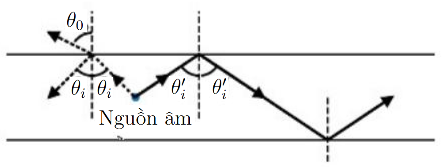
\includegraphics[width=0.53\textwidth]{images/Hinh 7b (S).png}
\end{figure}

\noindent \textbf{4.} Khi khoảng cách là tương đối lớn, ta cần xét đến hình dạng của Trái Đất. Ở đây ta có thể chia vấn đề thành 4 trường hợp, tuỳ thuộc vào vị trí của nguồn âm và đầu thu:
\begin{enumerate}
  \item[A.] Khi nguồn âm và đầu thu đều nằm trong tầng đối lưu, sẽ không có hiện tượng phản xạ toàn phần xảy ra. Vì không có hiện tượng phản xạ, đầu thu chỉ có thể thu được âm thanh nếu không bị Trái Đất cản trở, đường đi của sóng âm được biểu diễn bằng mũi tên $A$ trong hình 7c. Trong trường hợp này, khoảng cách phát hiện tối đa là:
        \begin{equation*}
          l_{1}=\sqrt{(R_{e}+h_{1})^{2}-R_{e}^{2}}\approx2\sqrt{2R_{e}h_{1}}\approx\SI{714}{\kilo\metre}
        \end{equation*}
        Vì vậy, trong trường hợp này, ta không thể phát hiện được nguồn âm ở cách xa hàng nghìn kilomet.
  \item[B.] Nguồn âm ở tầng đối lưu và đầu thu ở tầng bình lưu, do không xảy ra hiện tượng phản xạ, ta chỉ có thể thu được âm khi không bị Trái Đất cản trở, đường đi của sóng âm trong trường hợp này được biểu diễn bằng mũi tên $B$ trong hình 7c. Trong trường hợp này, khoảng cách phát hiện xa nhất sẽ không vượt quá khoảng cách từ một điểm trên đỉnh của tầng dối lưu, dọc theo tiếp tuyến của mặt phân cách đến một điểm trên đỉnh tầng bình lưu, nghĩa là nó sẽ không vượt quá:
        \begin{equation*}
          l_{1}=\sqrt{(R_{e}+h_{2})^{2}-R_{e}^{2}}-\sqrt{(R_{e}+h_{1})^{2}-R_{e}^{2}}\approx2\sqrt{2R_{e}h_{2}} + 2\sqrt{2R_{e}h_{1}}\approx\SI{862}{\kilo\metre}
        \end{equation*}
        Vì vây, trong trường hợp này, ta không thể phát hiện được nguồn âm ở cách xa hàng nghìn kilomet.
  \item[C.] Nguồn âm và đầu thu cùng ở tầng bình lưu. Vì khoảng cách giữa hai bề mặt khí quyển rất nhỏ so với bán kính Trái Đất nên sóng âm bị phản xạ toàn phần trên mặt này cũng sẽ phản xạ toàn phần trên bề mặt kia. Do đó, âm thanh có góc tới nhỏ trong tầng bình lưu có thể bị phản xạ liên tục quả hai mặt phân cách và sẽ bị giới hạn trong tầng bình lưu, do đó nó sẽ tiếp tục là truyền như được biểu diễn trên hình 7d. Vì vậy, trong trường hợp này ta có thể thu được âm thanh ở cách xa vài nghìn kilomet.
  \item[D.] Nguồn âm ở tầng bình lưu và khí cầu ở tầng đối lưu, tương tự như trường hợp $A$ và $B$, ta không thể thu được âm thanh ở cách xa vài nghìn kilomet.
\end{enumerate}

\begin{figure}[h]
  \centering
  \begin{minipage}{6cm}
    \centering
    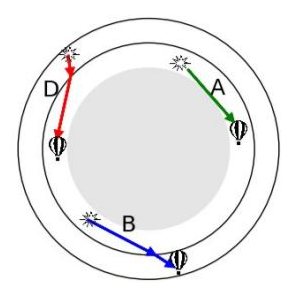
\includegraphics[width=1.1\textwidth]{images/Hinh 7c (S) .png}
    \begin{center}
      \figurename{ 7c}
    \end{center}
  \end{minipage}
  \hfil
  \begin{minipage}{6cm}
    \centering
    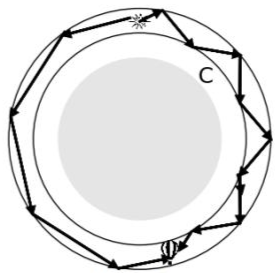
\includegraphics[width=1\textwidth]{images/Hinh 7d (S).png}
    \vspace{1mm}
    \begin{center}
      \figurename{ 7d}
    \end{center}
  \end{minipage}
\end{figure}






